\documentclass[11pt, a4paper]{article}
\usepackage[utf8]{inputenc}
\usepackage[T1]{fontenc}
\usepackage[norsk]{babel}
\usepackage{hyperref}
\usepackage{fancyvrb}
\usepackage{marginnote}

\usepackage{tgheros}
\renewcommand*\familydefault{\sfdefault}

\usepackage{xspace}
\newcommand{\TikZ}{Ti\textit{k}Z\xspace}

\usepackage{tikz}
\usepackage{circuitikz}

\usepackage{amsmath}

\usetikzlibrary{automata}
\usetikzlibrary{shapes}
\usetikzlibrary{mindmap}
\usetikzlibrary{calendar}

\title{Oppgaver i \TikZ}
\author{Veronika Heimsbakk \\ veronika.heimsbakk@acando.no}
\date{}


\begin{document}

\maketitle


\section{Former}
Gjør deg kjent med de forskjellige nøkkelordene for former i \TikZ. Inkluder gjerne \TikZ-biblioteket \texttt{shapes} ved å bruke \texttt{\textbackslash usetikzlibrary\{shapes\}}.

\begin{center}
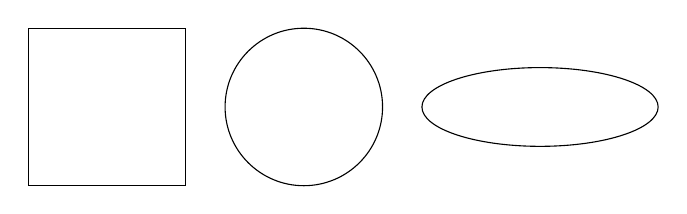
\begin{tikzpicture}
\draw(0,0) rectangle (2,2);
\draw(3.5,1) circle (1);
\draw(6.5,1) ellipse (1.5 and 0.5);
\end{tikzpicture}
\end{center}

\begin{center}
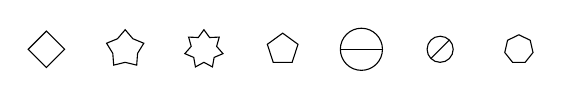
\begin{tikzpicture}
\node[diamond, draw=black] () at (0,0) {};
\node[star, star points=5, draw=black] () at (1,0) {};
\node[star, star points=7, draw=black] () at (2,0) {};
\node[regular polygon, regular polygon sides=5, draw=black] () at (3,0) {};
\node[circle split, draw=black] () at (4,0) {};
\node[forbidden sign, draw=black] () at (5,0) {};
\node[regular polygon, regular polygon sides=7, draw=black] () at (6,0) {};
\end{tikzpicture}
\end{center}

\section{Farger}
Prøv deg frem med forskjellige farger på strek og fyll for formene i forrige oppgave. De tilgengelige fargene vi har er:
\begin{verbatim}
red violet purple magenta pink white green lime olive orange yellow b
rown blue cyan teal lightgray gray darkgray black
\end{verbatim}
Opsjonene for fyll er \texttt{fill=<farge>} og for strek er \texttt{draw=<farge>}.

\begin{center}

\begin{tikzpicture}
\shade[top color=orange, bottom color=orange!50](0,0) rectangle (2,2);
\shade[inner color=pink, outer color=white](3.5,1) circle (1);
\shade[inner color=magenta, outer color=violet](6.5,1) ellipse (1.5 and 0.5);
\end{tikzpicture}
\end{center}

\begin{center}

\begin{tikzpicture}
\node[diamond, draw=black, fill=cyan] () at (0,0) {};
\node[star, star points=5, draw=teal, ultra thick] () at (1,0) {};
\node[star, star points=7, fill=orange] () at (2,0) {};
\node[regular polygon, regular polygon sides=5, draw=darkgray, fill=brown] () at (3,0) {};
\node[circle split, draw=black, fill=lime] () at (4,0) {};
\node[forbidden sign, draw=black, fill=red] () at (5,0) {};
\node[regular polygon, regular polygon sides=7, fill=pink] () at (6,0) {};
\end{tikzpicture}
\end{center}

\newpage


\section{Trær}
Bygg et tre med fem noder, hvor tre av nodene er løvnoder.

\begin{center}
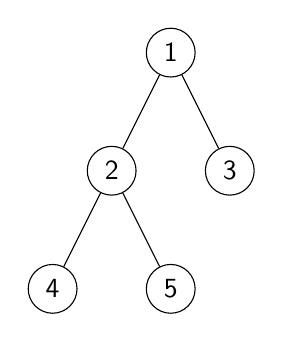
\begin{tikzpicture}[every node/.style={circle, draw=black}]
\node {1}
	child { node {2}
		child { node {4} }
		child { node {5} }
	}
	child { node {3} }
;
\end{tikzpicture}
\end{center}

\section{Trær forts.}
Legg til to noder til i treet, hvor minst ett av de er barn av node \tikz \node[circle, draw=black] {3};. Juster gjerne \texttt{sibling distance} for å unngå at nodene overlapper.

\paragraph{Eksempel}
\begin{center}
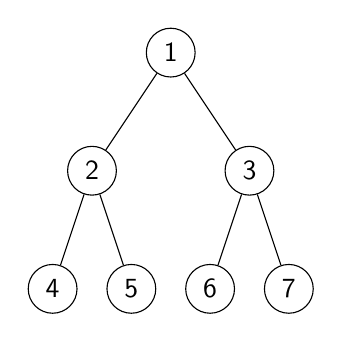
\begin{tikzpicture}[every node/.style={circle, draw=black},
					level 1/.style={sibling distance=20mm},
					level 2/.style={sibling distance=10mm}]
\node {1}
	child { node {2}
		child { node {4} }
		child { node {5} }
	}
	child { node {3} 
		child { node {6} }
		child { node {7} }
	}
;
\end{tikzpicture}
\end{center}

\section{Trær med \texttt{tikzset}}
Lag et \texttt{tikzset} som definerer rød-svarte noder. Her trenger vi å definere en stil for \textit{røde noder}, \textit{svarte noder} og \textit{null-noder}. Husk at \texttt{tikzset} defineres utenfor selve \texttt{tikzpicture}.

\paragraph{Eksempel}
\tikzset {
	treenode/.style={align=center},
	black_node/.style={treenode, circle, white, font=\bfseries, draw=black, fill=black},
	red_node/.style={treenode, circle, red, draw=red, very thick},
	null_node/.style={treenode, rectangle, draw=black, minimum width=3mm, minimum height=3mm}
}
\begin{center}
\begin{tikzpicture}[->,thick, level 1/.style={level distance=10mm},
					level 2/.style={level distance=10mm, sibling distance=5mm}]
\node[black_node] {2}
	child { node[red_node] {1} 
		child { node[null_node] {}}
		child { node[null_node] {}}
	}
	child { node[red_node] {3} 
		child { node[null_node] {}}
		child { node[null_node] {}}
	}
;
\end{tikzpicture}
\end{center}

\section{\texttt{tikzstyle}}
Klarer du å løse forrige oppgave med å bruke \texttt{tikzstyle} istedenfor \texttt{tikzset}?

\section{Plassering av noder og kanter}
Hvordan kan vi tegne følgende graf ved å benytte oss av opsjonene for plassering av noder og tegne kanter mellom disse nodene? Husk at det er mulig å gi navn og plassering til nodene ved å bruke \texttt{\textbackslash node (<navn>) at (x, y) \{<merkelapp\};}.
\begin{center}
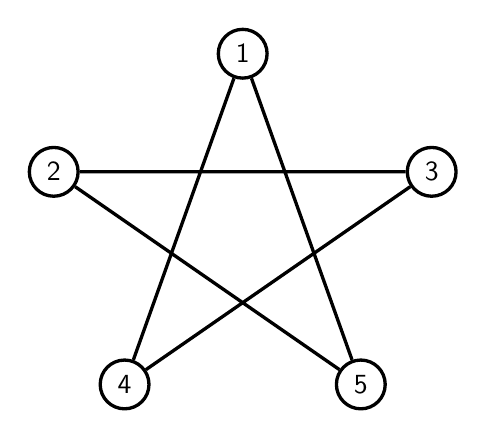
\begin{tikzpicture}[very thick, every node/.style={circle, draw=black}]
\node (1) at (0,0) {1};
\node (2) at (-2.4,-1.5) {2};
\node (3) at (2.4,-1.5) {3};
\node (4) at (-1.5, -4.2) {4};
\node (5) at (1.5,-4.2) {5};

\draw (1) -- (4) -- (3) -- (2) -- (5) -- (1);
\end{tikzpicture}
\end{center}

\section{Automater}
Benytt \TikZ-biblioteket \texttt{automata} til å tegne en automat. Du bestemmer selv hvilken. Her er et eksempel.

\paragraph{Eksempel}
\begin{center}
\scalebox{0.8}{
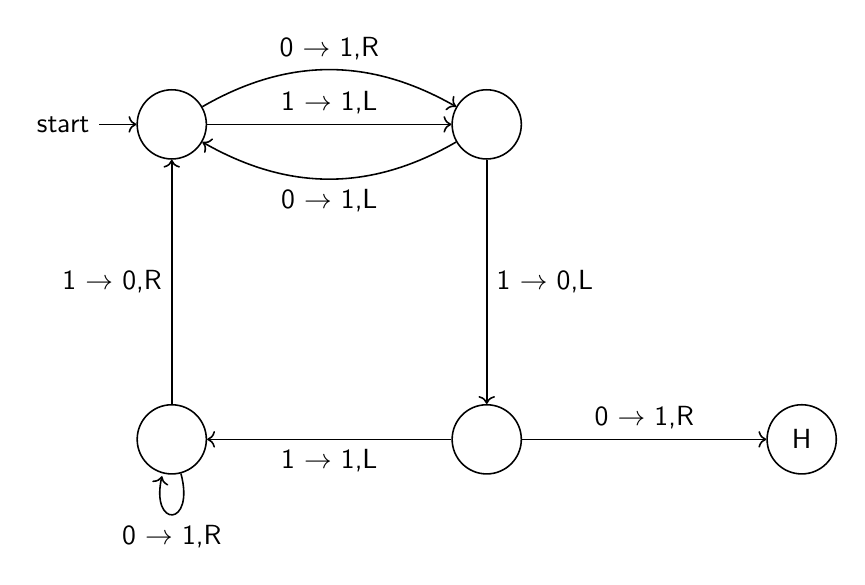
\begin{tikzpicture}[->,auto,node distance=4cm,line width=0.2mm]
  \node[initial,state] 		(A)            			{};
  \node[state] 			(B) [below of=A]   	{};
  \node[state] 			(C) [right of=A]    		{};
  \node[state] 			(D) [below of=C] 		{};
  \node[state]         		(E) [right of=D] 		{H};

  \path 	(A) edge node 				{1 $\rightarrow$ 1,L} 		(C)
		(A) edge [bend left] node 		{0 $\rightarrow$ 1,R} 		(C)
		(C) edge [bend left] node 		{0 $\rightarrow$ 1,L} 		(A)
		(B) edge node 				{1 $\rightarrow$ 0,R} 		(A)
		(B) edge [loop below] node 	{0 $\rightarrow$ 1,R} 		(B)
		(D) edge node 				{1 $\rightarrow$ 1,L} 		(B)
		(C) edge node 				{1 $\rightarrow$ 0,L} 		(D)
		(D) edge node		 		{0 $\rightarrow$ 1,R} 		(E);
\end{tikzpicture}
}
\end{center}








\end{document}